\begin{table}[h]
\centering
% centering table
\begin{tabular}{l c c c}
% creating 10 columns
\multicolumn{4}{c}{ROUGE-1}\\
\hline
\hline
% inserting double-line
$\mathrm{System}$ & $\mathrm{Prec.}$ & $\mathrm{Recall}$ & $\mathrm{F}_1$\\
[0.5ex]
\hline
AP+Salience &          0.289   &    0.344  &  0.312  \\
AP+Salience TR &       0.278   &    0.342  &  0.303 \\
AP    &         0.246   &    0.285  &  0.263 \\
HAC     &        0.238   &    0.276  &  0.255 \\
Rank    &        0.229   &    0.271  &  0.247 \\
\hline % inserts single-line
\end{tabular}
~\\[1ex]
~\\
\begin{tabular}{l c c c}
% creating 10 columns
\multicolumn{4}{c}{ROUGE-2}\\
\hline
\hline
% inserting double-line
$\mathrm{System}$ & $\mathrm{Prec.}$ & $\mathrm{Recall}$ & $\mathrm{F}_1$\\[0.5ex]
\hline
AP+Salience & 0.047 &     0.056 &   0.051 \\
AP+Salience TR & 0.044  &    0.054 &  0.047 \\
AP & 0.033  &    0.038 &  0.035 \\
HAC & 0.031  &    0.035 &  0.034 \\
Rank & 0.031  &    0.037 &  0.034 \\
\hline % inserts single-line
\end{tabular}
\caption{System ROUGE performance.} % title name of the table
\label{tab:rouge}
\end{table}


\subsection{ROUGE}

Table~\ref{tab:rouge} shows our results for the retrospective evaluation using ROUGE. 
Both versions of AP+Salience show improvement on ngram precision and recall over the 
baselines. This improvement is statistically significant at the $\alpha = .01$ level
using the Wilcoxon signed-rank test. Additionally, AP+Salience's improvement over
AP+Salience TR in recall and F-measure is also statistically significant at the same level.

AP+Salience maintains its performance above the baselines over time as well. Table~\ref{fig:trouge}
shows the ROUGE-1 performance over time. Within the initial days of the event, recall is 
competitive amongst system. However, both AP+Salience variants are able to achieve higher
precision early on.  

\subsection{Nugget Evaluation}

Figure~\ref{fig:nuggets} shows the average gain across a range of 
similarity thresholds, where thresholds closer to 1 are more conservative
estimates. The ranking of the systems remains relatively constant across the 
sweep with 
AP+Salience and AP+Salience TR attaining comparable performance, as well
as beating all baseline systems.
Predicting salience in general is helpful for keeping a summary on topic as
the Rank by salience approach out performs the clustering only approaches
on average gain.

When looking at the comprehensiveness of the summaries AP outperforms
both AP+Salience variants. The compromise encoded in the AP+Salience objective
function, between being representitive and being salient, is seen clearly here
where the performance of the AP+Salience methods is lower bounded by 
the salience focused Rank
system and upper bounded by the clustering only AP system.



\subsection{Feature Ablation}

\begin{figure}
    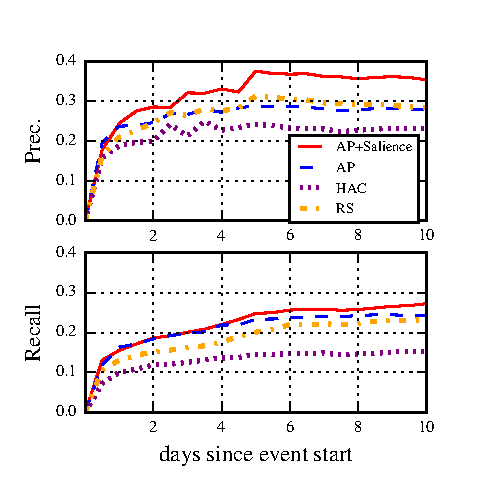
\includegraphics[]{rouge-time.eps}
\caption{System ROUGE-1 performance over time.}
\label{fig:trouge}
\end{figure}

\begin{figure}
  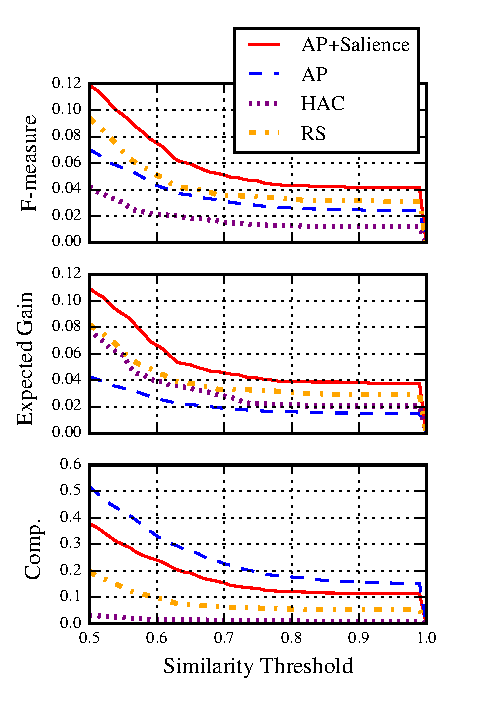
\includegraphics[]{nuggets-metrics.eps}
\caption{Avg. Gain and Comprehensiveness performance.}
\label{fig:nperf}
\end{figure}

